% --------------------------------------------------------------------------- %
% !TEX encoding = UTF-8 Unicode
% !TEX TS-program = pdflatex
% !TEX root = main.tex
% !TEX spellcheck = en-EN
% --------------------------------------------------------------------------- %

\chapter{Review of Falling-Snow Models}
	In this chapter the theoretical framework behind a general drag coefficient model will be explained and a review of the available models in literature will be proposed. 
	
	Recalling from \sref{sec: NonSphericalParticles}, the formula used for these models is the following:
	\begin{equation}
		c_D = c_D(Re, \text{model}, \text{parameters})
	\end{equation}
	
	The main physical quantities used in this definition will now be clarified, referring the reader to the nomenclature for a comprehensive list of the names of the other variables and the terms appearing in the equations.
	The drag coefficient is defined as:
	\begin{equation}
		c_D = \dfrac{F_D}{\frac{1}{2} \rho u^2 S_{\perp}}
	\end{equation}
	with $ F_D $ being the drag force, $ \rho $ being the fluid density and $ S_{\perp} $ being the projection of the area of the particle on a plane normal to the velocity vector ($ \underline{u} $).
	
	The models provide a constitutive relation for the drag coefficient, using non-dimensional parameters such as the Reynolds Number ($ Re $) and other quantities describing the shape of the particle and its orientation.
	 
	The characteristic dimension of the particle ($ \dv $) which appears in the definition of the Reynolds Number and the drag coefficient ($ c_D $) is defined as the diameter of the volume-equivalent sphere. Furthermore, the Reynolds number of the particle is based on the relative velocity of the fluid w.r.t. the particle:
	\begin{equation}
		Re = \dfrac{u \ \dv}{\nu} \qquad \text{with: } \qquad u := || \underline{u}_f - \underline{u}_p ||
	\end{equation}

	The parameter mainly used to describe the shape of the particle is the \textit{sphericity}, that is the ratio between the surface area of the
	volume-equivalent sphere and the area of the actual particle:
	\begin{equation}
		\Phi = \dfrac{\pi \ \dv^2} {A_{\textup{p}}}
	\end{equation}
	This is a common element between various models, while the choice of a parameter to describe the particle orientation is broader, thus each one of those will be presented in relation wit its model.
	
	\section{Chhabra review}
		In 1999 Chhabra et al. published a review article on non-spherical particles \cite{ChhabraEtAl-1999}. They evaluated a selection of the most used correlations methods using experimental results culled from 19 independent studies, consisting of 1900 data points with wide ranges of physical and kinematics conditions as: sphericity, $ 0.09 $ to $ 1 $ and the Reynolds number ranging from $ 10^{-4} $ to$  5 \cdot 10^{5} $. The performances of the methods were evaluated by calculating the mean and maximum error with respect to a certain shape category (sphere, cube, cylinder and so on) and considering the overall data set. 
		The best method appeared to be that of Ganser \cite{Ganser-1993} which will be discussed in the following section.
		Yet, a more significant contribution of this article was the definition
		of a new standard for a non-spherical particle model, stating that a good correlation formula must account for information on 2 main aspect: \textit{shape} of the particle (sphericity) and \textit{orientation} of the particle. 
		
		In the following sections the Ganser model, alongside with two more recent one, will be reviewed and compared on the basis of the literature that is available. 
		
	\section{Ganser - 1993}
		The Ganser model \cite{Ganser-1993} comes from empirical correlations of the general drag formula by Haider and Levenspiel \cite{HaiderLevenspiel-1989}:
		\begin{equation}
			c_D = \frac{24}{Re} (1 + A Re^B) + \dfrac{C}{1 + \frac{D}{Re}}
		\end{equation}
	
		It relies on the notion that a good $ c_D $ formula must involve a dependence on at least two shape descriptors. Using similarity arguments and dimensional analysis, Ganser showed that knowledge of the Stokes' shape factor ($ K_1 $) and of the Newton's shape factor ($ K_2 $) is sufficient for accurate prediction of the drag over a large range of Reynolds number. 
		Geometric shape descriptors such as sphericity are used	to model $ K_1 $ and $ K_2 $ and not $ c_D $, directly.
		
		The basic assumption in this paper is that every isolated particle experiences a Stokes’ regime where the drag is proportional to velocity and a Newton’s regime where the drag is proportional to the square of velocity. 
		
		In addition, it is possible to extract shape and orientation factors	from the behaviour of the particle in the Stokes’s and Newton’s regimes with dimensional analysis. Then, the way a particle behaves in these two regimes can be used to predict the drag for a large range of Reynolds numbers.
		
		The general definition for the Stokes' shape factor reads:
		\begin{equation}
			K_1 = \left( \frac{1}{3} \frac{\dn}{\dv} + \frac{2}{3} \Phi^{-\frac{1}{2}} \right)^{-1} -2.25 \frac{\dv}{D_{\textup{tube}}} 
		\end{equation}
		where the importance of both the shape and the orientation of the particle in the viscous regime ($ Re \ll 1 $) is measured by the \textit{sphericity} ($ \Phi $) and the ratio between the \textit{normal diameter} and the \textit{volume diameter} ($ \dn / \dv $), as already stated by Leith \cite{Leith-1987}, who first introduced the Stokes' shape factor.
		Since we will consider only snowflakes falling in an open environment, the second term is negligible, as $ D_{\textup{tube}} \rightarrow \infty $.
		
		Thompson and Clark \cite{ThompsonClark-1991} defined the Newton's shape factor as the ratio between the drag coefficient of a particle of a certain shape and the drag coefficient of a sphere, both at Reynolds number of 10 000, following the argument that, at high Reynolds (Newton's regime), the $ c_D $ is approximately constant.
		From this observation, Ganser derived the following formula for the Newton's shape factor:
		\begin{equation}
			K_2 = 10^{1.8148 (-log(\Phi))^{0.5743}}
		\end{equation}
		
		The final version of the model is function of the \textit{generalized} Reynolds number ($ Re K_1 K_2 $) and reads:
		\begin{equation}
			c_D = K_2 \left( \frac{24}{Re K_1 K_2} (1 + 0.1118 (Re K_1 K_2)^{0.6567}) + \frac{0.4305}{1 + \frac{3305}{Re K_1 K_2}}\right) 
		\end{equation}
	
				
	\section{H\"{o}lzer and Sommerfeld - (2008)}
		The model by H\"{o}ltzer and Sommerfeld \cite{HoltzerSommerfeld-2008} is, in effect, an interpolation of previous models coming from an extensive literature review. The coefficients of their final formula are tuned on a collection of over two thousands experimental data. The $ c_D $ values used are summarized in \fref{fig: LitReviewHS}, featuring spheres, disk and plates, lengthwise spheroids and streamline bodies, isometric particles such as cubes, tetrahedrons and octahedrons and irregularly shaped particles such as minerals.
		
		Similarly to Ganser, they used different models for the Stokes' and the Newton's regime. The Stokes' region is characterized by an inverse proportionality between the drag coefficient and the Reynolds number. The formula used is the one suggested by Leith \cite{Leith-1987}:
		\begin{equation}
			c_D = \frac{8}{Re} \frac{1}{\sqrt{\Phi_{\perp}}} + \frac{16}{Re} \frac{1}{\Phi}
			\label{eq: Leith}
		\end{equation}
		where the particle orientation is measured by the crosswise sphericity ($ \Phi_{\perp} $), which is defined in \eref{eq: Crosswise} as the ratio between the cross-sectional area of the volume-equivalent sphere w.r.t. the cross-sectional area of the actual particle projected on a plane perpendicular to the velocity vector ($ A_{\textup{p}, \perp} $).
		\begin{equation}
			\Phi_{\perp} = \dfrac{\frac{\pi}{4}\ \dv^2} {A_{\textup{p}, \perp}}
			\label{eq: Crosswise}
		\end{equation}
		
		The first term in \eref{eq: Leith} stands for the pressure or form drag, associated with the size of the projected cross-sectional area, and the second term represents the friction drag, associated with the size of the surface area. Correlation with experimental data showed that the use of the lengthwise sphericity ($ \Phi_{/\!/} $) instead of $ \Phi_{\perp} $ in \eref{eq: Leith} leads to a better approximation of the $ c_D $ in the Stokes region. The lengthwise sphericity is defined in \eref{eq: Lengthwise} as the ratio between the cross-sectional area of the volume-equivalent sphere and the difference between half the surface area ($ A_{\textup{p}} $) and the mean longitudinal (i.e. parallel to the direction of relative flow) projected cross-sectional area of the actual particle ($ \bar{A}_{\textup{p},/\!/} $). Since $ A_{\textup{p},/\!/} $ depends on the angle of view, an arithmetic average over an entire revolution is used.
		\begin{equation}
			\Phi_{/\!/} = \dfrac{\frac{\pi}{4}\ \dv^2} {\Delta A} \qquad \text{with: } \qquad \Delta A = \dfrac{A_{\textup{p}}}{2} - \bar{A}_{\textup{p},/\!/}
		\end{equation}

		For the Newton's regime a two different models are used. The former
		represents the friction drag of lengthwise particles (small cross-sectional area). The mathematical model describing this phenomenon is, according to Blasius' theory:
		\begin{equation}
			c_D = 1.327 \cdot 2 \left(\frac{8}{9}\right)^{\frac{1}{4}} \pi^{\frac{1}{4}} \left(\frac{\text{depth}}{\text{length}}\right)^{\frac{1}{4}} \frac{1}{\Phi^{\frac{3}{4}}} \frac{1}{\sqrt{Re}}
			\label{eq: Blasius}
		\end{equation}
		which, for square plates reduces to:
		\begin{equation}
			c_D = 3.43 / (\Phi^{\frac{3}{4}} \sqrt{Re})
			\label{eq: SimpleBlasius}
		\end{equation}
		and this simplified version will be used.
		
		The latter derives from the study of Tran-Cong et at \cite{TranCongEtAl-2004} and represent the behaviour of isometric and cross-wise oriented bodies. The $ c_D $ os such particles in the Newton's regime is almost solely determined by form drag, in particular it is approximately proportional to the reciprocal of crosswise sphericity. Merging this study with the literature by Ganser and Leith, H\"{o}ltzer and Sommerfeld proposed the following formula for isometric and crosswise oriented particles at high Reynolds number:
		\begin{equation}
			c_D = 0.4210^{0.4(-\log \Phi)^{0.2}} \frac{1}{\Phi_{\perp}}
			\label{eq: TranCong}
		\end{equation}

		The correlation formula for the $ c_D $ over the entire range of $ Re  $ results from the addition of \cref{eq: Leith, eq: SimpleBlasius, eq: TranCong} \red{FIX EQUATION REF}:
		\begin{equation}
			c_D = \frac{8}{Re} \frac{1}{\sqrt{\Phi_{/\!/}}} 
			    + \frac{16}{Re} \frac{1}{\sqrt{\Phi}} 
			    + \frac{3}{\sqrt{Re}} \frac{1}{\Phi^{\frac{3}{4}}} 
			    + 0.4210^{0.4(-\log \Phi)^{0.2}} \frac{1}{\Phi_{\perp}}
			\label{eq: HS}
		\end{equation}
	
		In the same paper, they also derive a simplified model of similar performance, in terms of accuracy w.r.t.\ all the available data, depending on two parameters only, namely $\Phi$ and $\Phi_{\perp}$, which reads:
		\begin{equation}
			c_D = \frac{8}{Re} \frac{1}{\sqrt{\Phi_{\perp}}} 
			    + \frac{16}{Re} \frac{1}{\sqrt{\Phi}} 
			    + \frac{3}{\sqrt{Re}} \frac{1}{\Phi^{\frac{3}{4}}} 
			    + 0.4210^{0.4(-\log \Phi)^{0.2}} \frac{1}{\Phi_{\perp}}
			\label{eq: SimpleHS}
		\end{equation}
		

























		\begin{figure}
			\centering
			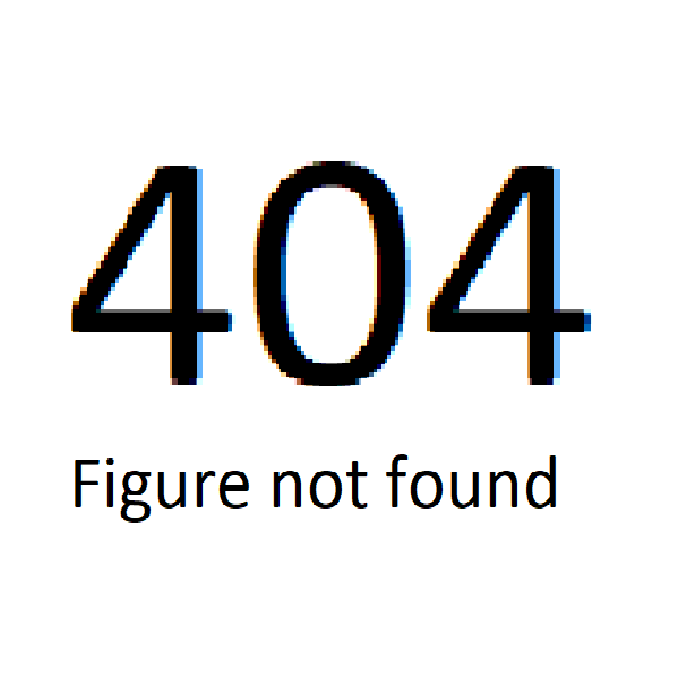
\includegraphics[width=\linewidth]{404notFound.png}
			\caption{Drag coefficient of different shaped particles as function of the Reynolds number. Data from the literature review of Holtzer and Sommerfeld. \cite{HoltzerSommerfeld-2008}}
			\label{fig: LitReviewHS}
		\end{figure}

%		Description of the model and it's simplified form. 
		
	\section{Heymsfield and Westbrook - (2010)}
		Description of the model ans why it doesn't work.

	\section{Model comparison}
		comparison between the models and justification of my choice.
		Comparison H\&S - Ganser: sensitivity study on the parameters of both models and why H\&S better suits the experimental curves of snow
		
		(+ "cite" the ICE GENESIS results proving that this model is the better one)		
		
	\section{Terminal Velocity calculation}
		Equation for the terminal velocity of a particle: how to calculate every term starting from the diameter and the shape parameters
	
